\documentclass[paper=a4, fontsize=11pt]{scrartcl} 

\usepackage[T1]{fontenc} 
\usepackage[english]{babel}
\usepackage{amsmath,amsfonts,amsthm}
\usepackage{lipsum}
\usepackage{graphicx}
\usepackage{float}
  \floatplacement{figure}{H}
  \floatplacement{table}{H}
  
\usepackage{sectsty} 
\allsectionsfont{\centering \normalfont\scshape} 

\usepackage{fancyhdr} % Custom headers and footers
\pagestyle{fancyplain} % Makes all pages in the document conform to the custom headers and footers
\fancyhead{} % No page header - if you want one, create it in the same way as the footers below
\fancyfoot[L]{} % Empty left footer
\fancyfoot[C]{} % Empty center footer
\fancyfoot[R]{\thepage} % Page numbering for right footer
\renewcommand{\headrulewidth}{0pt} % Remove header underlines
\renewcommand{\footrulewidth}{0pt} % Remove footer underlines
\setlength{\headheight}{13.6pt} % Customize the height of the header

\numberwithin{equation}{section} % Number equations within sections (i.e. 1.1, 1.2, 2.1, 2.2 instead of 1, 2, 3, 4)
\numberwithin{figure}{section} % Number figures within sections (i.e. 1.1, 1.2, 2.1, 2.2 instead of 1, 2, 3, 4)
\numberwithin{table}{section} % Number tables within sections (i.e. 1.1, 1.2, 2.1, 2.2 instead of 1, 2, 3, 4)

\setlength\parindent{0pt} % Removes all indentation from paragraphs - comment this line for an assignment with lots of text

\usepackage[labelformat=empty]{caption}
\usepackage{color}
\usepackage{listings}
\lstset{ %
language=bash,                % choose the language of the code
basicstyle=\footnotesize,       % the size of the fonts that are used for the code
numbers=left,                   % where to put the line-numbers
numberstyle=\footnotesize,      % the size of the fonts that are used for the line-numbers
stepnumber=1,                   % the step between two line-numbers. If it is 1 each line will be numbered
numbersep=5pt,                  % how far the line-numbers are from the code
backgroundcolor=\color{white},  % choose the background color. You must add \usepackage{color}
showspaces=false,               % show spaces adding particular underscores
showstringspaces=false,         % underline spaces within strings
showtabs=false,                 % show tabs within strings adding particular underscores
frame=single,           % adds a frame around the code
tabsize=2,          % sets default tabsize to 2 spaces
captionpos=b,           % sets the caption-position to bottom
breaklines=true,        % sets automatic line breaking
breakatwhitespace=false,    % sets if automatic breaks should only happen at whitespace
escapeinside={\%*}{*)}          % if you want to add a comment within your code
}

%----------------------------------------------------------------------------------------
%	TITLE SECTION
%----------------------------------------------------------------------------------------

\newcommand{\horrule}[1]{\rule{\linewidth}{#1}} % Create horizontal rule command with 1 argument of height

\title{	
\normalfont \normalsize 
\textsc{Computational Science - ITB} \\ [25pt] % Your university, school and/or department name(s)
\horrule{0.5pt} \\[0.4cm] % Thin top horizontal rule
\large Analisis Numerik Lanjut - Genetic Algorithm\\ % The assignment title
%\horrule{2pt} \\[0.5cm] % Thick bottom horizontal rule
}

\author{\small{Ridlo W. Wibowo || 20912009}} % Your name

\date{\normalsize\today} % Today's date or a custom date

\begin{document}

\maketitle % Print the title

\large \textbf{Soal.}\\
Buatlah algoritma genetik untuk menyelesaikan masalah optimasi. Terapkan pada kasus berikut:
\begin{itemize}
\item Cari minimum fungsi
\begin{equation*}
x^{2} - 10 \cos(2 \pi x) + 10 \hspace{1.5cm} -5 \leq x \leq 5
\end{equation*}
\item Cari maksimum fungsi
\begin{equation*}
x \sin(10 \pi x) + 1 \hspace{1.5cm} -1 \leq x \leq 2
\end{equation*}
\item Cari minimum fungsi
\begin{equation*}
f(x_{i}) = \sum_{i=1}^{2}(x_{i} - 10 \cos(2 \pi x_{i}) + 10) \hspace{1.5cm} -5 \leq x_{i} \leq 5
\end{equation*}
\item Cari minimum fungsi
\begin{equation*}
f(x_{1}, x_{2}) = \frac{1}{2}(x_{1}^{4} - 16x_{1}^{2} + 5x_{1}) + \frac{1}{2}(x_{2}^{4} - 16x_{1}^{2} + 5x_{2}) \hspace{0.5cm} -4 \leq x_{1}, x_{2} \leq 4
\end{equation*}
\end{itemize}

%\vspace{1.5cm}
\newpage
\large \textbf{Algoritma.}\\
Algoritma Genetika ini kami buat dengan menggunakan urutan proses sebagai berikut:
\begin{enumerate}
\item INPUT parameter, yaitu sebagai berikut:
\begin{itemize}
\item fungsi $f(x_{i})$ yang akan di cari maksimum atau minimumnya
\item batas bawah dan batas atas variabel
\item $k_{i}$ - ketelitian tiap variabel yang diinginkan (berapa angka dibelakang koma)
\item $n$ - banyaknya khromosom dalam populasi
\item $p_{c}$ - peluang terjadi persilangan
\item $p_{m}$ - peluang terjadi mutasi
\item $N$ - banyaknya iterasi 
\item $tipe$ - 0 untuk pencarian maksimum, 1 untuk pencarian minimum
\end{itemize}

\item GENERATE vektor biner, sesuai input $k$ (dihitung terlebih dahulu nilai $l$ setiap variabel lalu dijumlahkan), lalu simpan fitness terbaik dari populasi (inisiasi). Menghitung panjang vektor biner untuk $k$   adalah:
\begin{equation*}
l = \frac{\ln((b-a) 10^{k} + 1)}{\ln 2}
\end{equation*}
dengan $a$ dan $b$ adalah batas bawah dan atas variabel yang dicari.

\item Lakukan proses dibawah ini hingga $N$ kali:
\begin{enumerate}
\item SELECTION, roulette selection dengan menggunakan nilai $f(x)$ yang dinormalisasi (digeser agar positif semua). Untuk mengubah vektor biner menjadi nilai bilangan real dengan cara:
\begin{equation*}
x = a + (\sum_{k=0}^{l-1} b_{k} 2^{k})(\frac{b-a}{2^{l} - 1})
\end{equation*}

\item CROSSOVER, dilakukan dengan terlebih dahulu melakukan random untuk memperoleh calon orangtua yang akan disilangkan (menggunakan $p_{c}$).

\item MUTATION, dilakukan terhadap setiap bit dengan memperhatikan $p_{m}$. 

\item SAVE, cari nilai fitness terbaik di populasi, lalu bandingkan dengan nilai fitness terbaik yang sudah disimpan, jika lebih baik maka ganti.
\end{enumerate}
Langkah \textit{Selection} dan \textit{Save} memperhatikan $tipe$ masalah.
\item OUTPUT, nilai variabel dan nilai fungsi terbaik (maximum/minimum).
\end{enumerate}


\newpage
\large \textbf{Hasil.}\\
Parameter dibuat sama, yakni: $n = 50, N = 300, p_{c} = 0.8, p_{m} = 0.1, k = 5$
\begin{itemize}
\item minimum fungsi:
\begin{equation*}
x^{2} - 10 \cos(2 \pi x) + 10 \hspace{1.5cm} -5 \leq x \leq 5
\end{equation*}
\begin{figure}
	\centering
	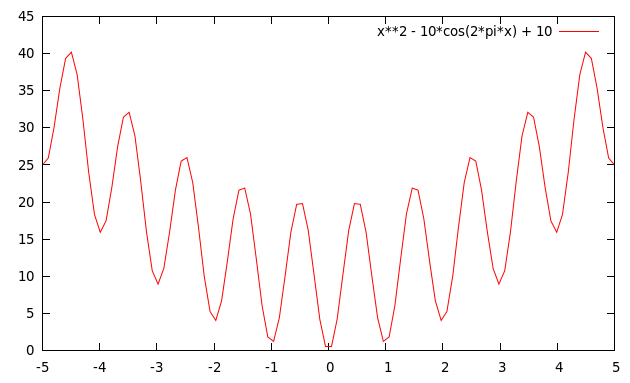
\includegraphics[width=0.45\textwidth]{kurva1.png}
	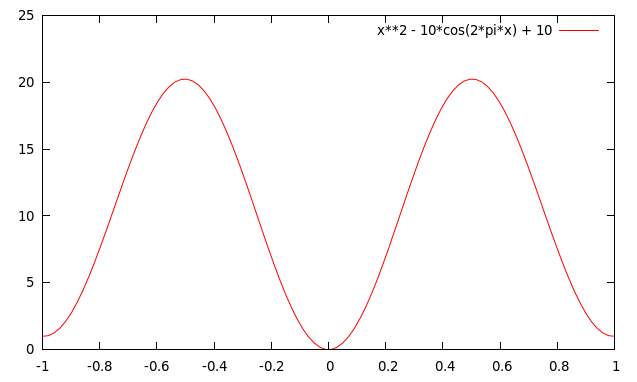
\includegraphics[width=0.45\textwidth]{kurva1zoom.png}
	\caption{Plot fungsi dan zoom disekitar $x = 0$}
\end{figure}

\begin{table}[ht]
\center
\begin{tabular}{c c c}
\hline
running & $x_{best}$ & $y_{best}$ \\ [0.5ex]
\hline 
run\_1 & 4.76838e-06 & 4.51092e-09 \\
run\_2 & 1.43051e-05 & 4.05983e-08 \\
run\_3 & 4.76838e-06 & 4.51092e-09 \\
run\_4 & -4.76838e-06 & 4.51092e-09 \\
run\_5 & 2.38419e-05 & 1.12773e-07 \\ [1ex]
\hline 
\end{tabular}
\end{table}
nilai minimum hasil run program berada di sekitar $x = 0$ dan $y = 0$.

\vspace{1.5cm}
\item maksimum fungsi:
\begin{equation*}
x \sin(10 \pi x) + 1 \hspace{1.5cm} -1 \leq x \leq 2
\end{equation*}
\begin{figure}
	\centering
	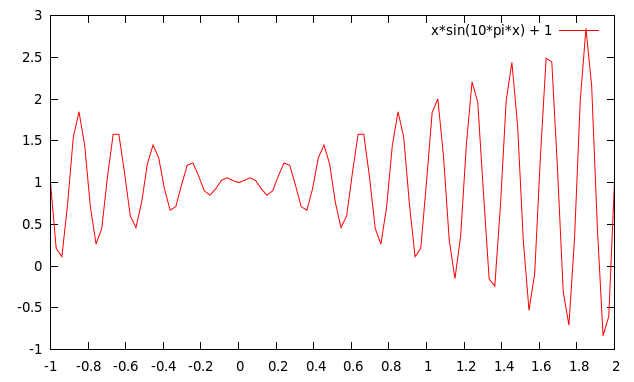
\includegraphics[width=0.45\textwidth]{kurva2.png}
	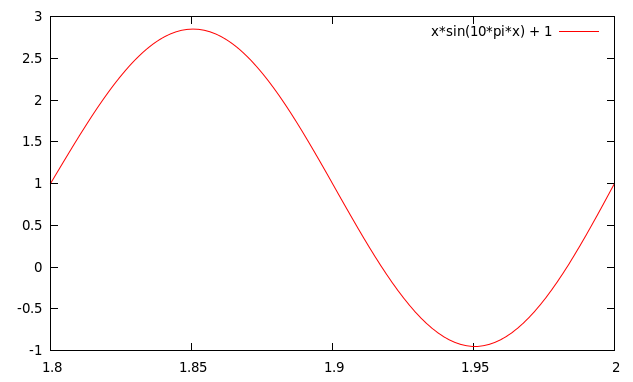
\includegraphics[width=0.45\textwidth]{kurva2zoom.png}
	\caption{Plot fungsi dan zoom disekitar $x = 1.9$}
\end{figure}

\begin{table}[ht]
\center
\begin{tabular}{c c c}
\hline
running & $x_{best}$ & $y_{best}$ \\ [0.5ex]
\hline 
run\_1 & 1.85062 & 2.85027 \\
run\_2 & 1.85054 & 2.85027 \\
run\_3 & 1.85056 & 2.85027 \\
run\_4 & 1.85052 & 2.85027 \\
run\_5 & 1.85035 & 2.85024 \\ [1ex]
\hline 
\end{tabular}
\end{table}
nilai maksimum hasil run program berada di sekitar $x = 1.85056$ dan $y = 2.85027$.

Contoh screenshot fitness:
\begin{figure}
	\centering
	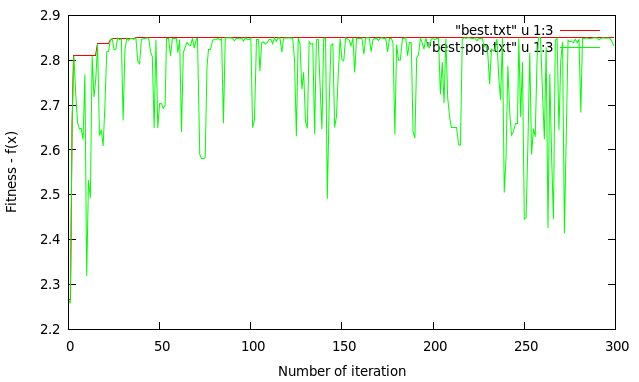
\includegraphics[width=0.7\textwidth]{fit1.png}
	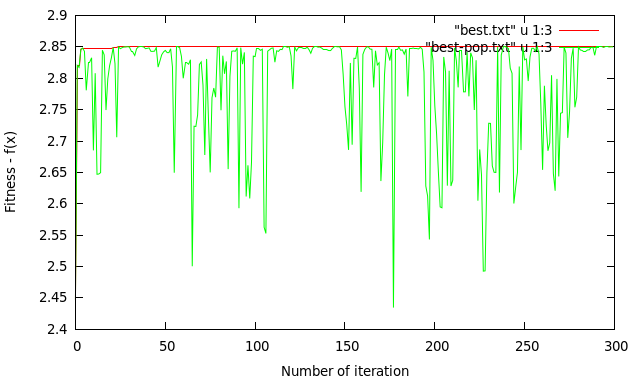
\includegraphics[width=0.7\textwidth]{fit2.png}
	\caption{Plot nilai fitness terhadap iterasi, merah menunjukkan fitness terbaik selama iterasi, dan hijau menunjukkan fitness terbaik untuk tiap step iterasi.}
\end{figure}


\vspace{1.5cm}
untuk kasus 2 dimensi digunakan $N = 500$.
\item minimum fungsi:
\begin{equation*}
f(x_{i}) = \sum_{i=1}^{2}(x_{i} - 10 \cos(2 \pi x_{i}) + 10) \hspace{1.5cm} -5 \leq x_{i} \leq 5
\end{equation*}
\begin{figure}
	\centering
	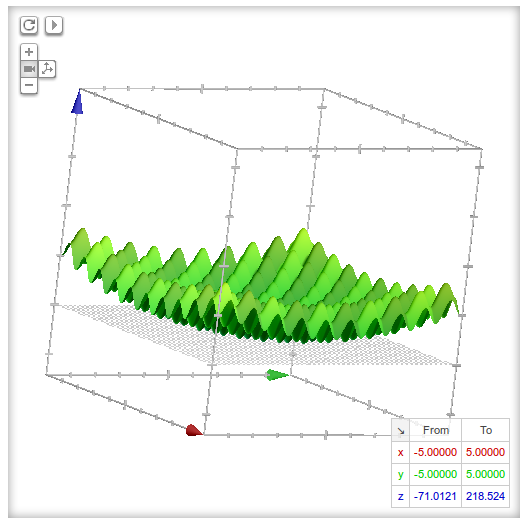
\includegraphics[width=0.7\textwidth]{kurva3.png}
	\caption{Plot fungsi, minima diduga ditengah kurva (0,0).}
\end{figure}

\begin{table}[ht]
\center
\begin{tabular}{c c c c}
\hline
running & $x_{1,best}$ & $x_{2,best}$ & $y_{best}$ \\ [0.5ex]
\hline 
run\_1 & -0.00058651 & 1.43051e-05  & 6.82863e-05 \\
run\_2 & 0.000195503 & -0.00110149  & 0.000248289 \\
run\_3 & -0.000519753 & -0.000414849  & 8.77374e-05 \\
run\_4 & 0.000681878 & -0.000300408  & 0.000110148 \\
run\_5 & -0.000414849 & -0.000262261 & 4.77887e-05 \\ [1ex]
\hline 
\end{tabular}
\end{table}
nilai minimum hasil run program berada di sekitar $x_{1} = 0, x_{2} = 0$, dan $f(x_{1},x_{2}) = 0$.


\vspace{1.5cm}
\item minimum fungsi:
\begin{equation*}
f(x_{1}, x_{2}) = \frac{1}{2}(x_{1}^{4} - 16x_{1}^{2} + 5x_{1}) + \frac{1}{2}(x_{2}^{4} - 16x_{1}^{2} + 5x_{2}) \hspace{0.5cm} -4 \leq x_{1}, x_{2} \leq 4
\end{equation*}
\begin{figure}
	\centering
	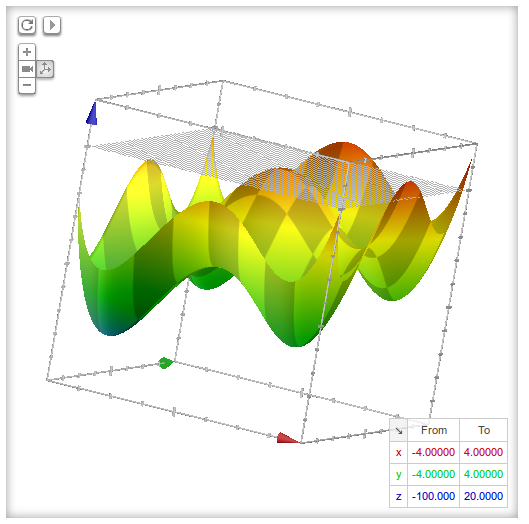
\includegraphics[width=0.7\textwidth]{kurva4.png}
	\caption{Plot fungsi, minima berada di daerah x-negatif dan y-negatif.}
\end{figure}

\begin{table}[ht]
\center
\begin{tabular}{c c c c}
\hline
running & $x_{1,best}$ & $x_{2,best}$ & $y_{best}$ \\ [0.5ex]
\hline 
run\_1 & -2.90181 & -2.90195  & -78.3322 \\
run\_2 & -2.9042 & -2.90497  & -78.3323 \\
run\_3 & -2.90234 & -2.9041  & -78.3323 \\
run\_4 & -2.90497 & -2.90304  & -78.3323 \\
run\_5 & -2.90357 & -2.90213  & -78.3323 \\ [1ex]
\hline 
\end{tabular}
\end{table}
nilai minimum hasil run program berada di sekitar $x_{1} = -2.903, x_{2} = -2.903$, dan $f(x_{1},x_{2}) = -78.3323$.



\end{itemize}

\newpage
\large \textbf{Lampiran Program.}\\
Kami sampaikan program untuk fungsi n-peubah saja.\\
\large Genetic Algorithm - untuk fungsi n-peubah:
\lstset{frameround=fttt}
\begin{lstlisting}
/********************************************************/
/* Simple Genetic Algorithm | N-dimensional Function    */
/* Copyleft (c) 2012. Ridlo W. Wibowo                   */
/********************************************************/

#include <iostream>
#include <stdlib.h>
#include <time.h>
#include <math.h>
#define _USE_MATH_DEFINES
using namespace std;

/***************** FUNCTION *********************/
/* mencari panjang vektor biner minimum */
double minL(double xi, double xf, int ko){
    return log((xf-xi) * pow(10., ko) + 1.)/log(2.);
}

/* random biner */
int brand(){ return rand()%2;}

/* random uniform 0-1 */
double unirand(){ return (double)rand()/(double)RAND_MAX;}

/* menghitung nilai real desimal */
double toDec(double xi, double xf, double li, int khrom[]){
    unsigned int sum = 0;
    for (int i=0;i<li;i++){ sum += khrom[i]*pow(2,i);}
    return (xi + sum*((xf-xi)/(pow(2,li) - 1)));
}

/****************** INPUT PARAMETER *********************/
/* jumlah variabel dalam fungsi */
int v = 2;

/* batas bawah dan atas fungsi */
int u=2*v;
//double bou['u'] = {-5., 5., -5., 5.}; // dua-dua
double bou['u'] = {-4., 4., -4., 4.}; 

/* ketelitian variable yang dicari (angka di belakang koma) */
int k['v'] = {5, 5}; 

/* fungsi */
double func(double x[]){
    return (0.5*(pow(x[0],4) - 16*pow(x[0],2) + 5*x[0]) + 0.5*(pow(x[1],4) - 16*pow(x[1],2) + 5*x[1]));
    //return (x[0]*x[0] - 10*cos(2.*M_PI*x[0]) + 10. + x[1]*x[1] - 10*cos(2.*M_PI*x[1]) + 10.);
}


/* jumlah khromosom dalam populasi */
int n = 50;

/* peluang terjadi cross-over */
double pc = 0.8;

/* peluang terjadi mutasi */
double pm = 0.1;

/* banyaknya iterasi */
int N = 500;

/* tipe optimasi, 0 = maximisasi, 1 = minimisasi */
int tipe = 1;



/************* GENETIC FUNCTION ************/
/* panjang vektor biner per variabel */
double lvar['v'];
/* panjang vektor biner total */
double l=0;
void vecLength(){
    for (int i=0;i<v;i++){
        lvar[i] = ceil(minL(bou[(2*i)],bou[(2*i)+1],k[i]));
        l += lvar[i];
    }
}

/* populasi */
int pop['n']['l'];
int induk['n']['l'];
int anak['n']['l'];

/* desimal, variabel dan fitness */
double x['n']['v']; double y['n'];
double xbest['v']; double ybest;
double xbestpop['v']; double ybestpop;

/* Generate Populasi Awal - biner */
void generate(){
    for (int i=0;i<n;i++){
        for (int j=0;j<l;j++){
            pop[i][j] = brand();
        }
    }
}

/* mencari nilai fitness */
void fitness(){
    int xpart['n']['v']['l'];
    for (int i=0;i<n;i++){
        int sum1 = 0;
        int sum2 = 0;
        for (int j=0;j<v;j++){
            sum2 = sum1+lvar[j];
            int o = 0;
            for (int w=sum1;w<sum2;w++){
                xpart[i][j][o] = pop[i][w];
                o += 1;
            }
            sum1 = sum2;
        }
    }
    
    for (int i=0;i<n;i++){
        for (int j=0;j<v;j++){
            x[i][j] = toDec(bou[(2*j)],bou[(2*j)+1],lvar[j],xpart[i][j]);
        }
        y[i] = func(x[i]);
    }
}

/* selection, Roulette-Wheel */
void selectRoulette(){
    fitness();
    double totFit = 0.;
    double cumFit['n'];
    double tot = 0.;
    double fit['n'];
    double rs;
    
    double mini = y[0];
    for (int i=1;i<n;i++){
        if (y[i] < mini){ mini = y[i];}
    }
    
    double geser = fabs(mini) + 1.;
    if (tipe == 0){
        for (int i=0;i<n;i++){ 
            fit[i] = (y[i] + geser);
         }
    } // maksimisasi
    else{for (int i=0;i<n;i++){ fit[i] = 1./(y[i]+geser);}} // minimisasi
    
    for (int i=0;i<n;i++){ totFit = totFit + fit[i];}
    for (int i=0;i<n;i++){ 
        cumFit[i] = tot + (fit[i]/totFit); 
        tot = cumFit[i];
    }

    for (int i=0;i<n;i++){
        rs = unirand();
        for (int j=0;j<n;j++){
            if (rs <= cumFit[j]){
                for (int w=0;w<l;w++){ induk[i][w] = pop[j][w];}
                break;
            }
        }
    }
}

/* cross-over */
void crossover(){
    int parent['n']['l'];
    int j=0;
    int p=0;
    for (int i=0;i<n;i++){
        if (unirand() <= pc){
            for (int w=0;w<l;w++){ parent[j][w] = induk[i][w];}
            j += 1;
        }
        else{
            for (int w=0;w<l;w++){ anak[p][w] = induk[i][w];}
            p += 1;
        }
    }
    if (j%2 == 1){ // kalau ganjil
        for (int w=0;w<l;w++){ anak[p][w] = parent[j-1][w];}
        p += 1;
        j -= 1;
    }
    for (int i=0;i<j/2;i++){
        int rk = 1 + rand()%((int)l-1);
        for (int q=0;q<rk;q++){
            anak[p+(2*i)][q] = parent[(2*i)][q];
            anak[p+(2*i+1)][q] = parent[(2*i+1)][q];
        }
        for (int r=rk;r<l;r++){
            anak[p+(2*i)][r] = parent[(2*i+1)][r];
            anak[p+(2*i+1)][r] = parent[(2*i)][r];
        }
    }
}

/* mutation */
void mutasi(){
    for (int i=0;i<n;i++){
        for (int j=0;j<l;j++){
            if (unirand() <= pm){
                if (anak[i][j] == 0){ anak[i][j] = 1;}
                else{ anak[i][j] = 0;}
            }
        }
    }
}

/* tukar populasi lama dengan yang baru */
void swapper(){
    for (int i=0;i<n;i++){
        for (int j=0;j<l;j++){
            pop[i][j] = anak[i][j];
        }
    }
}

/* simpan nilai terbaik di populasi */
void keep_the_best(){
    fitness();
    for (int i=0;i<v;i++){ xbestpop[i] = x[0][i];}
    ybestpop = y[0];
    if (tipe == 0){
        for (int i=1;i<n;i++){
            if (y[i] > ybestpop){
                for (int j=0;j<v;j++){ xbestpop[j] = x[i][j];}
                ybestpop = y[i];
            }
        }
    } else{
        for (int i=1;i<n;i++){
            if (y[i] < ybestpop){
                for (int j=0;j<v;j++){ xbestpop[j] = x[i][j];}
                ybestpop = y[i];
            }
        }
    }
    
    if (tipe == 0){
        if (ybestpop > ybest){ 
            ybest = ybestpop; 
            for (int j=0;j<v;j++){ xbest[j] = xbestpop[j];}
        }
    } else{
        if (ybestpop < ybest){
            ybest = ybestpop; 
            for (int j=0;j<v;j++){ xbest[j] = xbestpop[j];}
        }
    }
}

/* print best of the best */
void init(){
    keep_the_best(); 
    for (int j=0;j<v;j++){ xbest[j] = xbestpop[j];}
    ybest = ybestpop;
}
void print_best(){
    for (int j=0;j<v;j++){ cout << xbest[j] << " ";}
    cout << " " << ybest << endl;
}
void print_best_pop(){
    for (int j=0;j<v;j++){ cout << xbestpop[j] << " ";}
    cout << " " << ybestpop << endl;
} 

/* print real variable */
void print_real(){
    for (int i=0;i<n;i++){
        for (int j=0;j<v;j++){ cout << x[i][j] << " ";}
        cout << y[i] << endl;
    }
    cout << "\n\n";
}


/*************** FUNGSI-FUNGSI TESTING ******************/
/* print populasi */
void print_pop(){
    for (int i=0;i<n;i++){
        for (int j=0;j<l;j++){
            cout << pop[i][j] << " ";
        }
        cout << endl;
    }
    cout << endl;
}

/* print induk */
void print_induk(){
    for (int i=0;i<n;i++){
        for (int j=0;j<l;j++){
            cout << induk[i][j] << " ";
        }
        cout << endl;
    }
    cout << endl;
}

/* print anak */
void print_anak(){
    for (int i=0;i<n;i++){
        for (int j=0;j<l;j++){
            cout << anak[i][j] << " ";
        }
        cout << endl;
    }
    cout << endl;
}


/*************** MAIN ***************/
int main(){
    vecLength();
    srand(time(NULL));
    generate();
    init(); //print_pop();
    for (int s=0;s<N;s++){
        selectRoulette();
        //print_induk();  
        crossover();
        //print_anak();
        mutasi();
        //print_anak();
        swapper();
        keep_the_best();
        //print_real();
        //print_best_pop();
    }
    cout << "\nBest value: \n";
    print_best();
     
    return 0;
}
\end{lstlisting}

\end{document}














